\documentclass[12pt]{article}

% TEMPLATE DEFAULT PACKAGES
\usepackage{amssymb,amsmath,amsfonts,eurosym,geometry,ulem,graphicx,color,setspace,sectsty,comment,natbib,pdflscape,array,adjustbox}

% ADDED PACKAGES FOR THIS MANUSCRIPT
\usepackage{palatino,newtxmath,multirow,titlesec,threeparttable,tabu,booktabs,titlesec,threeparttable,mathtools,bm,bbm,subcaption,pdflscape,tcolorbox,mathrsfs}
% endfloat,

\usepackage{afterpage}
\usepackage[hyphens]{url}
\usepackage[margin=1cm]{caption}

\usepackage[draft]{hyperref}
\newcommand{\tim}{$\,\times\,$}
% FIGURES & TABLES CAPTION STYLING
\captionsetup[figure]{labelfont={bf},name={Figure},labelsep=period}
\captionsetup[table]{labelfont={bf},name={Table},labelsep=period}

% SECTION TITLE SETTINGS
\titlelabel{\thetitle.\enskip}
\titleformat*{\section}{\large\bfseries}
\titleformat*{\subsection}{\normalsize\bfseries}

% COLUMN TYPES
\newcolumntype{L}[1]{>{\raggedright\let\newline\\\arraybackslash\hspace{0pt}}m{#1}}
\newcolumntype{C}{>{\centering\arraybackslash}p{5.2em}}
\newcolumntype{D}{>{\centering\arraybackslash}p{5em}}
\newcolumntype{R}[1]{>{\raggedleft\let\newline\\\arraybackslash\hspace{0pt}}m{#1}}


% MARGINS AND SPACING
\normalem
\geometry{left=1.1in,right=1.1in,top=1.0in,bottom=1.0in}
\setlength{\parskip}{2.5pt}

% SPECIAL CELL 
\newcommand{\specialcell}[2][c]{%
	\begin{tabular}[#1]{@{}l@{}}#2\end{tabular}}

% NO INDENT ON FOOTNOTES
\usepackage[hang,flushmargin]{footmisc}

\begin{document}



\vspace{0mm}
\begin{table}[h!]
\centering
\caption{Housing Project Areas Description}\label{table:projectdescriptives}
\vspace{0mm}
\begin{tabular}{l*{1}{cccccc}}
\toprule
  & \multicolumn{2}{c}{\textbf{All}}& \multicolumn{2}{c}{\textbf{Greenfield}}  & \multicolumn{2}{c}{\textbf{In-Situ}}   \\
  &Const. & Unconst. &Const. & Unconst.   & Const. & Unconst. \\
\midrule
 Number of Projects  & 172  & 145  & 43  & 20  & 27  & 29  \\ 
 Area (km2)  & 1.17  & 1.16  & 1.72  & 2.42  & 1.50  & 0.88  \\ 
 Median Construction Yr.  & 2006  & 2006  & 2006  & 2005  & 2004  & 2006  \\ 
 Delivered Houses  & 374  & 11  & 568  & 24  & 702  & 20  \\ 
 House Price in 1 km (R$^\dagger$)  & 188,441  & 218,635  & 194,214  & 186,841  & 179,596  & 208,570  \\ 
 Distance to CBD$^\ddagger$ (km)  & 32.5  & 27.7  & 40.5  & 39.9  & 32.6  & 30.6  \\ 

\bottomrule
\multicolumn{7}{l}{\scriptsize Const. refers to constructed projects and unconst. refers to unconstructed projects.}\\[-.5em]
\multicolumn{7}{l}{\scriptsize $^*$Calculated from {\it expected} completion dates using Gauteng National Treasury budget reports.}\\[-.5em]
\multicolumn{7}{l}{\scriptsize $^\dagger$ The USD averaged to about 7.70 Rands during the 2001-2011 period.}\\[-.5em]
\multicolumn{7}{l}{\scriptsize $^\ddagger$Measured as the average minimum distance with respect to Johannesburg and Pretoria CBDs. } \\[-.5em]
%\multicolumn{7}{l}{\scriptsize City includes projects whose centroids are within 30.4 km of their nearest CBD.} \\[-.5em]
%\multicolumn{7}{l}{\scriptsize Suburb includes projects whose centroids are further than 30.4 km from their nearest CBD.}
\end{tabular}
\end{table} 



\begin{figure*}
        \centering
   %     \caption[ Pre-Period Housing Densities in Constructed and Unconstructed Projects Areas ]
  %      {\small Pre-Period Densities} 
        %\vspace{2mm}
        \begin{subfigure}[b]{0.48\textwidth}
                    \caption[Network2]%
            {{\footnotesize \textbf{All Projects} pre-period formal raw data}}    
            \label{fig:prefor}
            \centering
            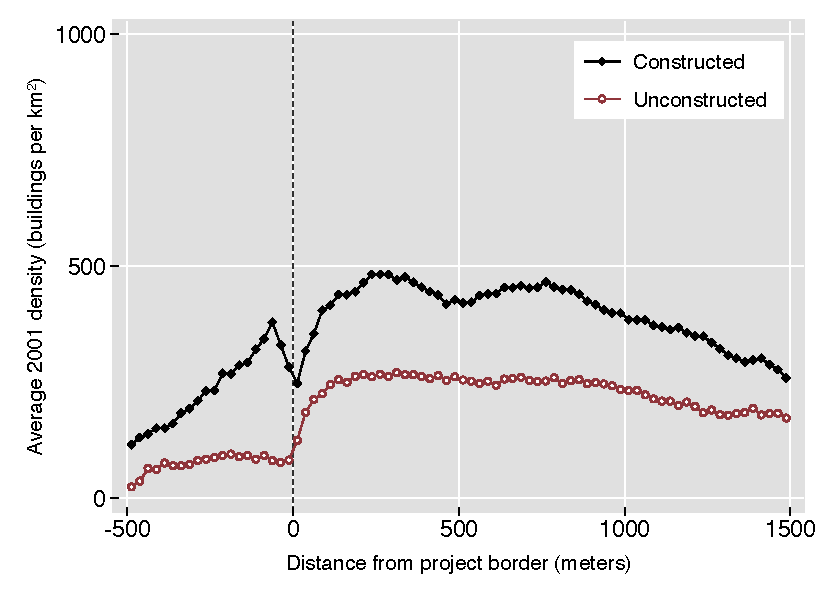
\includegraphics[width=\textwidth,trim={0.3cm .3cm 0.1cm 0cm}, clip=true]{figures/bblu_for_pre_means_4_spk.pdf}

        \end{subfigure}
        \hfill
        \begin{subfigure}[b]{0.48\textwidth}  
                    \caption[]%
            {{\footnotesize \textbf{All Projects} pre-period informal  raw data}}      
            \label{fig:preinf}
            \centering 
            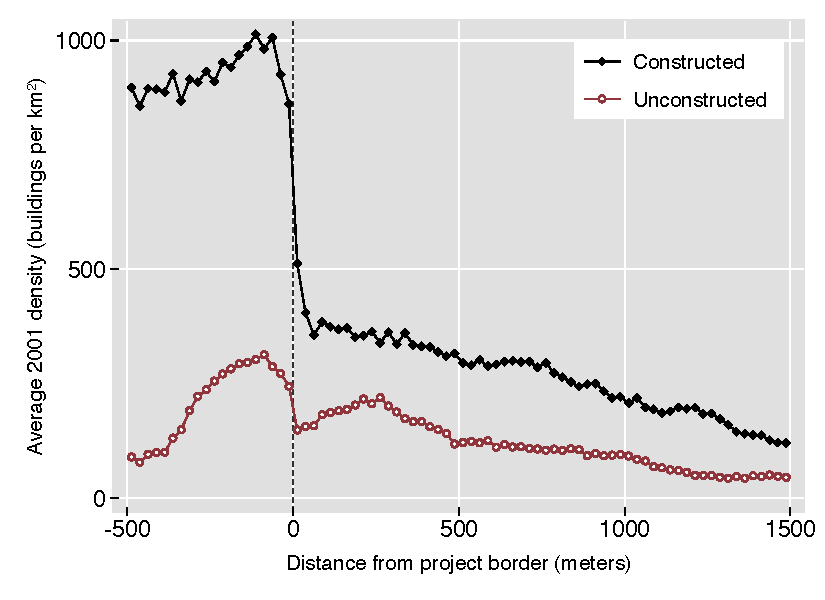
\includegraphics[width=\textwidth,trim={0.3cm .3cm 0.1cm 0cm}, clip=true]{figures/bblu_inf_pre_means_4_spk.pdf}

        \end{subfigure}
        \begin{subfigure}[b]{0.48\textwidth}
                    \caption[Network2]%
            {{\footnotesize \textbf{Greenfield} pre-period formal  raw data}}    
            \label{fig:prefor}
            \centering
            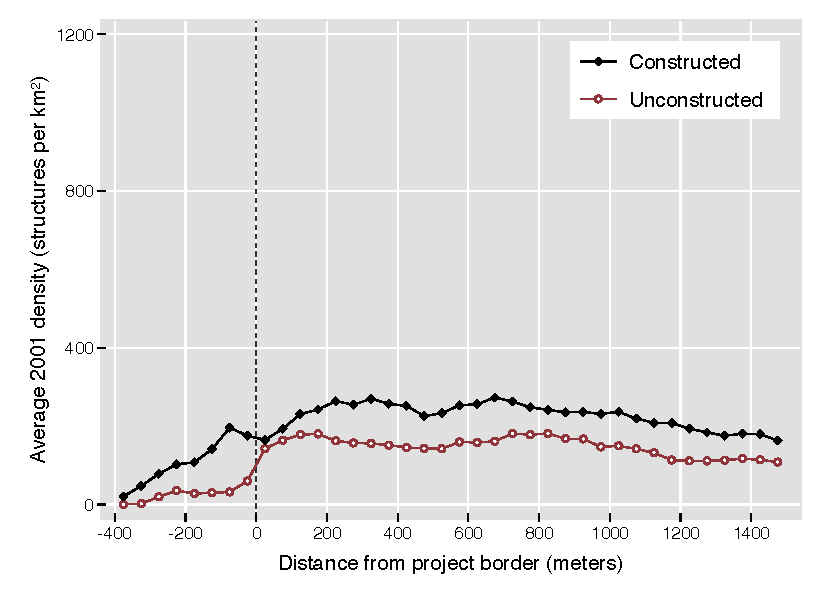
\includegraphics[width=\textwidth,trim={0.3cm .3cm 0.1cm 0cm}, clip=true]{figures/bblu_for_pre_means_4_1_spk.pdf}

        \end{subfigure}
        \hfill
        \begin{subfigure}[b]{0.48\textwidth}  
                    \caption[]%
            {{\footnotesize \textbf{Greenfield} pre-period informal  raw data}}     
            \label{fig:preinf}
            \centering 
            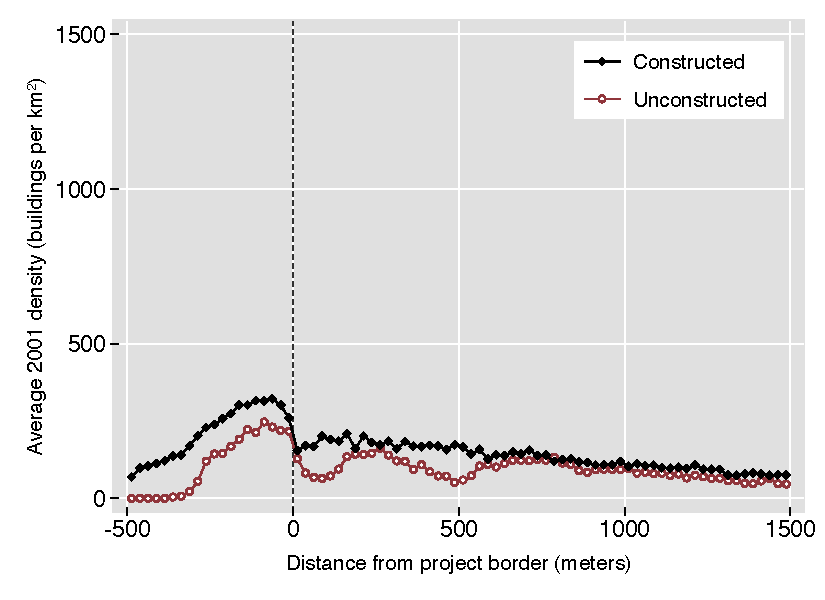
\includegraphics[width=\textwidth,trim={0.3cm .3cm 0.1cm 0cm}, clip=true]{figures/bblu_inf_pre_means_4_1_spk.pdf}

        \end{subfigure}
        \begin{subfigure}[b]{0.48\textwidth}
                    \caption[Network2]%
            {{\footnotesize \textbf{In-Situ} pre-period formal  raw data}}   
            \label{fig:prefor}
            \centering
            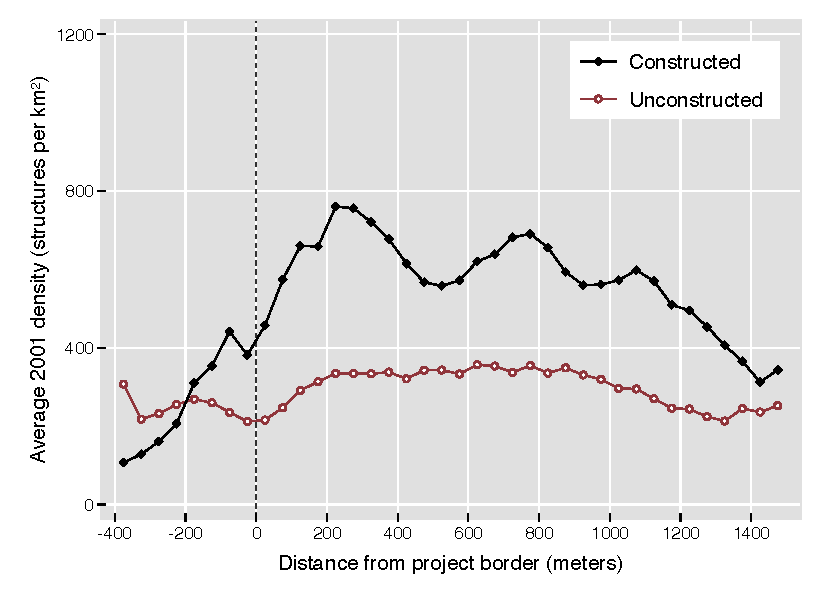
\includegraphics[width=\textwidth,trim={0.3cm .3cm 0.1cm 0cm}, clip=true]{figures/bblu_for_pre_means_4_2_spk.pdf}

        \end{subfigure}
        \hfill
        \begin{subfigure}[b]{0.48\textwidth}  
                    \caption[]%
            {{\footnotesize \textbf{In-Situ} pre-period informal  raw data}}     
            \label{fig:preinf}
            \centering 
            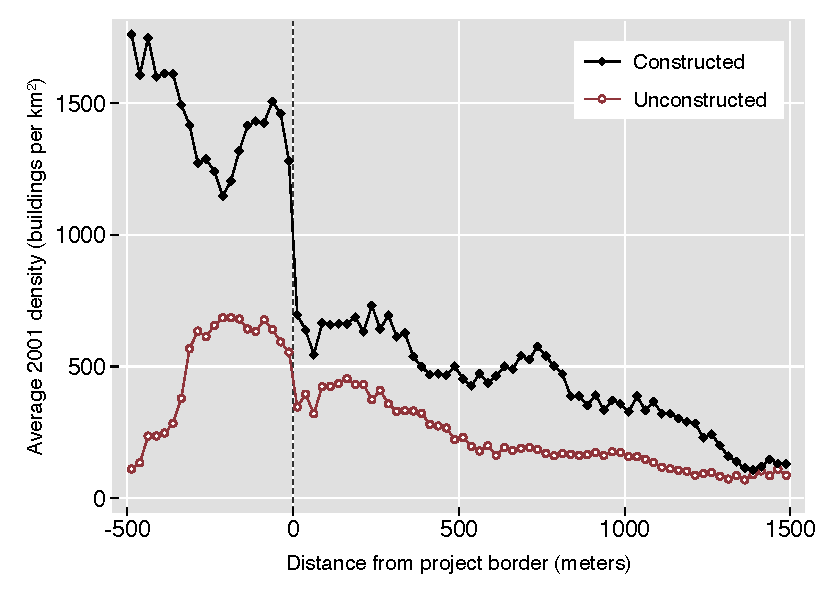
\includegraphics[width=\textwidth,trim={0.3cm .3cm 0.1cm 0cm}, clip=true]{figures/bblu_inf_pre_means_4_2_spk.pdf}

        \end{subfigure}
        \begin{subfigure}[b]{0.48\textwidth}
                    \caption[Network2]%
            {{\footnotesize \textbf{Other} pre-period formal  raw data}}   
            \label{fig:prefor}
            \centering
            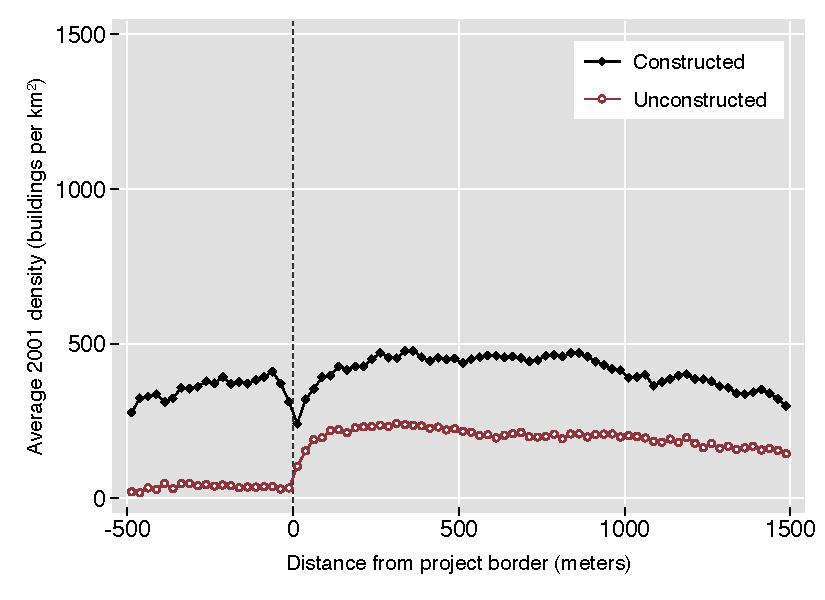
\includegraphics[width=\textwidth,trim={0.3cm .3cm 0.1cm 0cm}, clip=true]{figures/bblu_for_pre_means_4_3_spk.pdf}

        \end{subfigure}
        \hfill
        \begin{subfigure}[b]{0.48\textwidth}  
                    \caption[]%
            {{\footnotesize \textbf{Other} pre-period informal  raw data}}      
            \label{fig:preinf}
            \centering 
            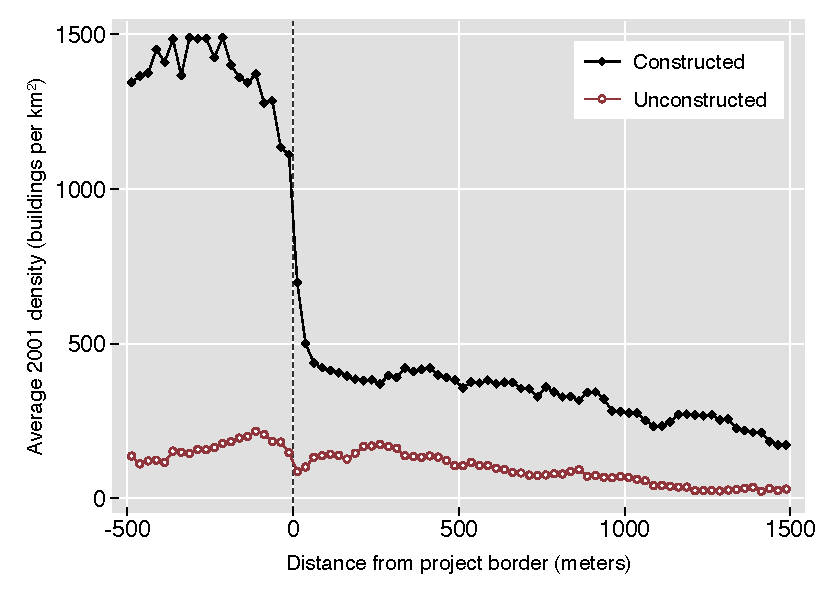
\includegraphics[width=\textwidth,trim={0.3cm .3cm 0.1cm 0cm}, clip=true]{figures/bblu_inf_pre_means_4_3_spk.pdf}

        \end{subfigure}
\end{figure*}


\begin{figure*}
        \centering
   %     \caption[ Pre-Period Housing Densities in Constructed and Unconstructed Projects Areas ]
  %      {\small Pre-Period Densities} 
        %\vspace{2mm}
        \begin{subfigure}[b]{0.48\textwidth}
                    \caption[Network2]%
            {{\footnotesize \textbf{All Projects} pre-period formal fe}}    
            \label{fig:prefor}
            \centering
            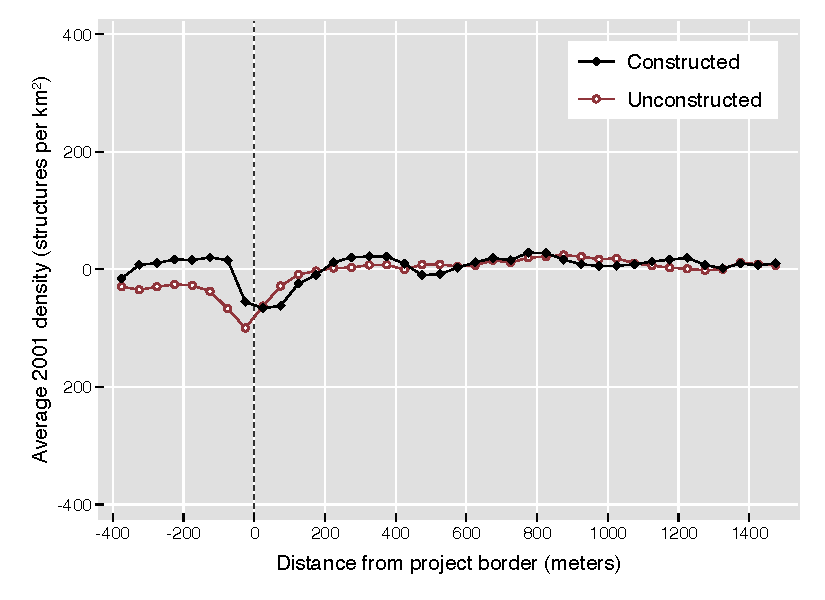
\includegraphics[width=\textwidth,trim={0.3cm .3cm 0.1cm 0cm}, clip=true]{figures/bblu_for_fe_pre_means_4_sp_postk.pdf}

        \end{subfigure}
        \hfill
        \begin{subfigure}[b]{0.48\textwidth}  
                    \caption[]%
            {{\footnotesize \textbf{All Projects} pre-period informal fe }}      
            \label{fig:preinf}
            \centering 
            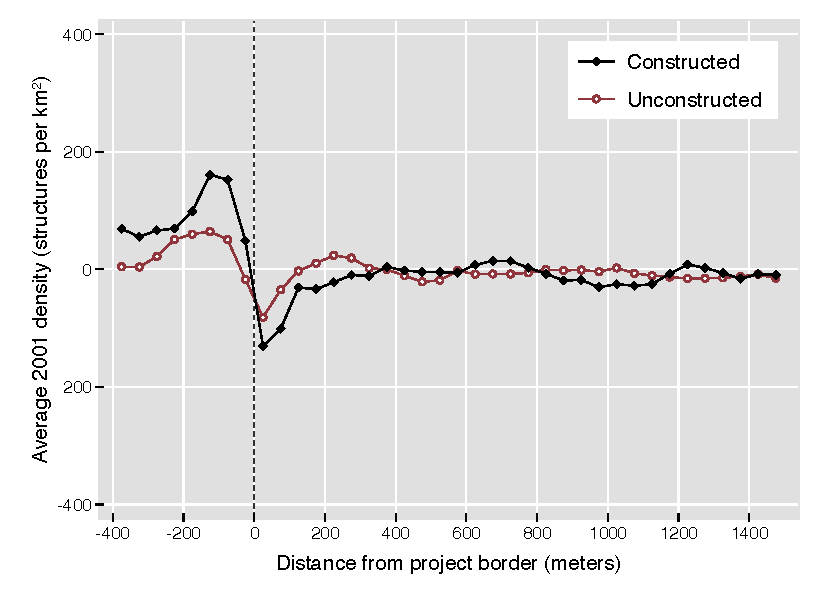
\includegraphics[width=\textwidth,trim={0.3cm .3cm 0.1cm 0cm}, clip=true]{figures/bblu_inf_fe_pre_means_4_sp_postk.pdf}

        \end{subfigure}
        \begin{subfigure}[b]{0.48\textwidth}
                    \caption[Network2]%
            {{\footnotesize \textbf{Greenfield} pre-period formal  fe }}    
            \label{fig:prefor}
            \centering
            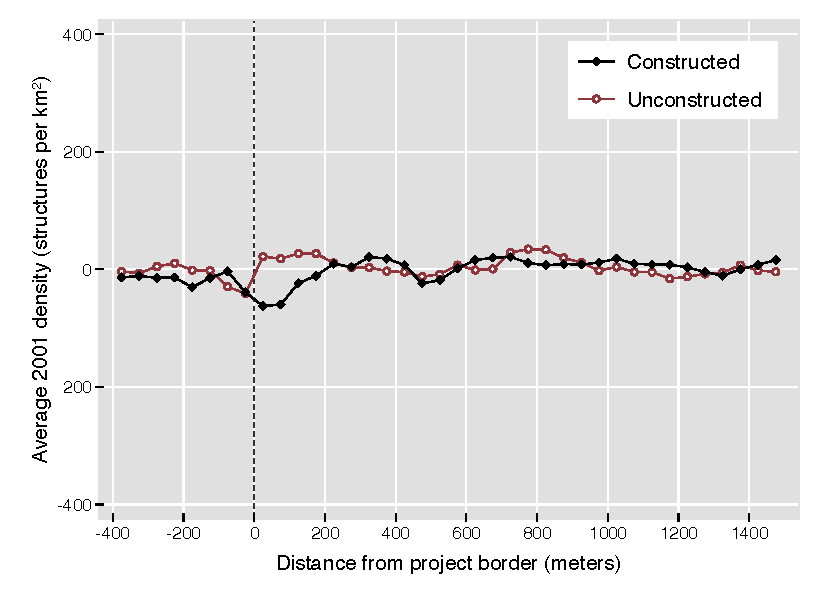
\includegraphics[width=\textwidth,trim={0.3cm .3cm 0.1cm 0cm}, clip=true]{figures/bblu_for_fe_pre_means_4_1_sp_postk.pdf}

        \end{subfigure}
        \hfill
        \begin{subfigure}[b]{0.48\textwidth}  
                    \caption[]%
            {{\footnotesize \textbf{Greenfield} pre-period informal fe }}     
            \label{fig:preinf}
            \centering 
            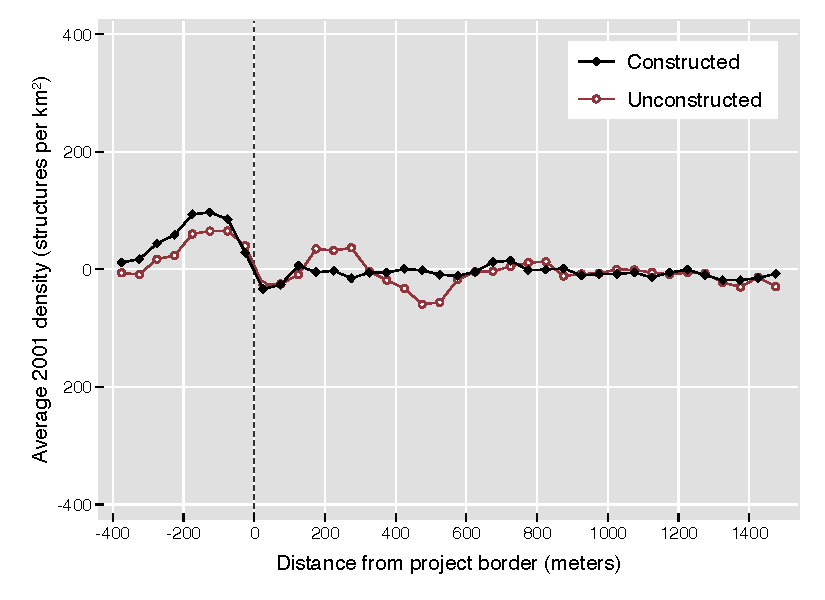
\includegraphics[width=\textwidth,trim={0.3cm .3cm 0.1cm 0cm}, clip=true]{figures/bblu_inf_fe_pre_means_4_1_sp_postk.pdf}

        \end{subfigure}
        \begin{subfigure}[b]{0.48\textwidth}
                    \caption[Network2]%
            {{\footnotesize \textbf{In-Situ} pre-period formal fe }}   
            \label{fig:prefor}
            \centering
            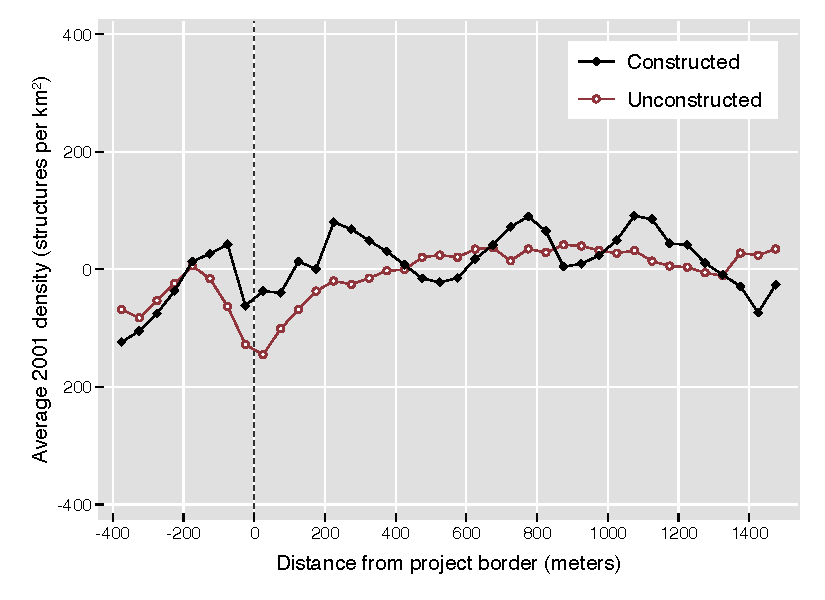
\includegraphics[width=\textwidth,trim={0.3cm .3cm 0.1cm 0cm}, clip=true]{figures/bblu_for_fe_pre_means_4_2_sp_postk.pdf}

        \end{subfigure}
        \hfill
        \begin{subfigure}[b]{0.48\textwidth}  
                    \caption[]%
            {{\footnotesize \textbf{In-Situ} pre-period informal fe }}     
            \label{fig:preinf}
            \centering 
            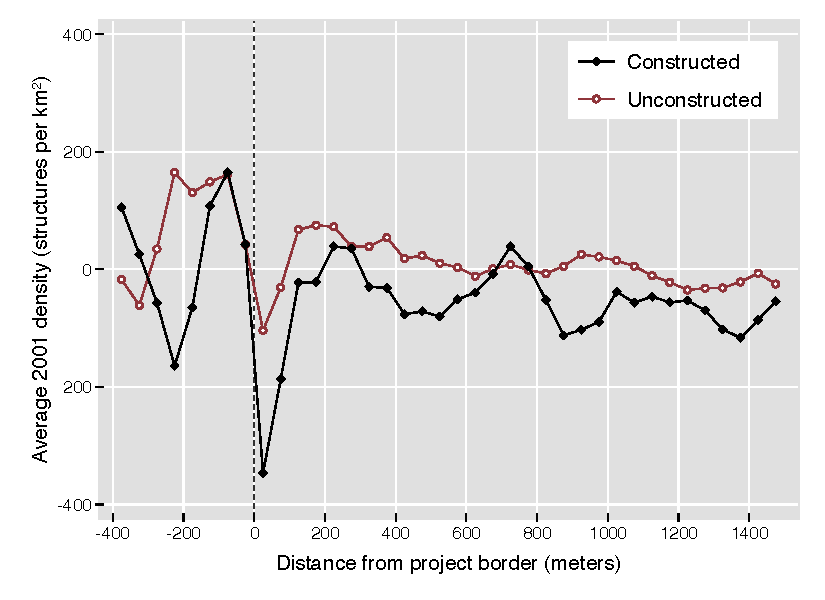
\includegraphics[width=\textwidth,trim={0.3cm .3cm 0.1cm 0cm}, clip=true]{figures/bblu_inf_fe_pre_means_4_2_sp_postk.pdf}

        \end{subfigure}
        \begin{subfigure}[b]{0.48\textwidth}
                    \caption[Network2]%
            {{\footnotesize \textbf{Other} pre-period formal fe }}   
            \label{fig:prefor}
            \centering
            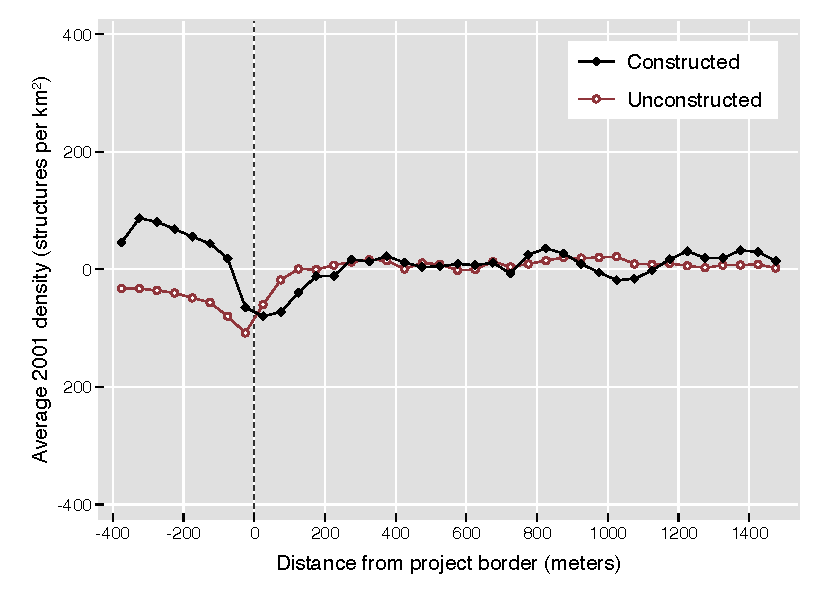
\includegraphics[width=\textwidth,trim={0.3cm .3cm 0.1cm 0cm}, clip=true]{figures/bblu_for_fe_pre_means_4_3_sp_postk.pdf}

        \end{subfigure}
        \hfill
        \begin{subfigure}[b]{0.48\textwidth}  
                    \caption[]%
            {{\footnotesize \textbf{Other} pre-period informal fe }}      
            \label{fig:preinf}
            \centering 
            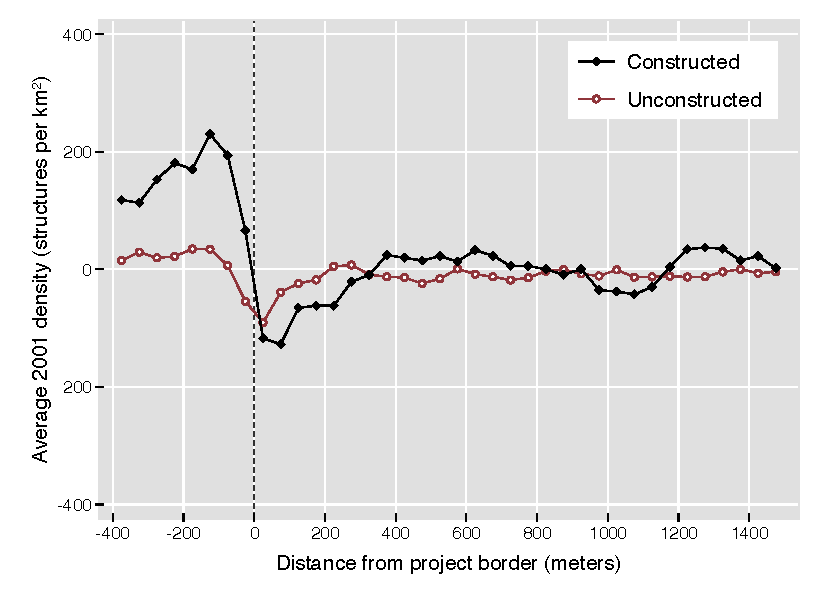
\includegraphics[width=\textwidth,trim={0.3cm .3cm 0.1cm 0cm}, clip=true]{figures/bblu_inf_fe_pre_means_4_3_sp_postk.pdf}

        \end{subfigure}
\end{figure*}








\begin{figure*}
        \centering
   %     \caption[ Pre-Period Housing Densities in Constructed and Unconstructed Projects Areas ]
  %      {\small Pre-Period Densities} 
        %\vspace{2mm}
        \begin{subfigure}[b]{0.48\textwidth}
            \caption[Network2]%
            {{\footnotesize \textbf{All Projects} changes formal raw data}}    
            \label{fig:prefor}
            \centering
            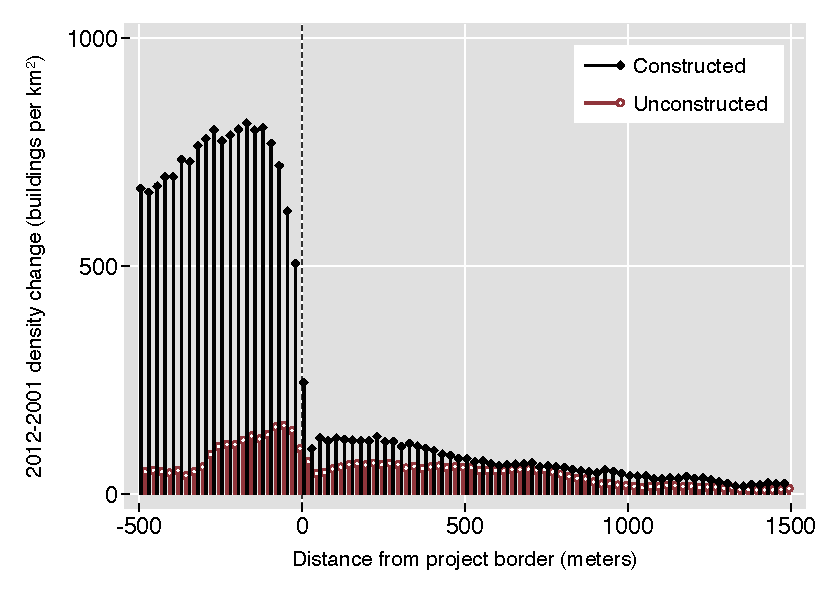
\includegraphics[width=\textwidth,trim={0.3cm .3cm 0.1cm 0cm}, clip=true]{figures/bblu_for_rawchanges_4_spk.pdf}

        \end{subfigure}
        \hfill
        \begin{subfigure}[b]{0.48\textwidth}  
                    \caption[]%
            {{\footnotesize \textbf{All Projects} changes informal  raw data}}      
            \label{fig:preinf}
            \centering 
            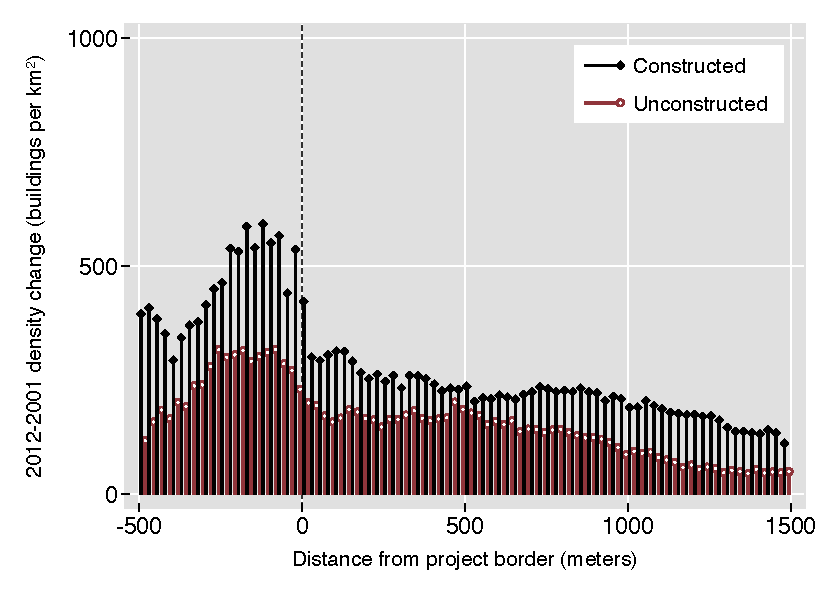
\includegraphics[width=\textwidth,trim={0.3cm .3cm 0.1cm 0cm}, clip=true]{figures/bblu_inf_rawchanges_4_spk.pdf}

        \end{subfigure}
        \begin{subfigure}[b]{0.48\textwidth}
                    \caption[Network2]%
            {{\footnotesize \textbf{Greenfield} changes formal  raw data}}    
            \label{fig:prefor}
            \centering
            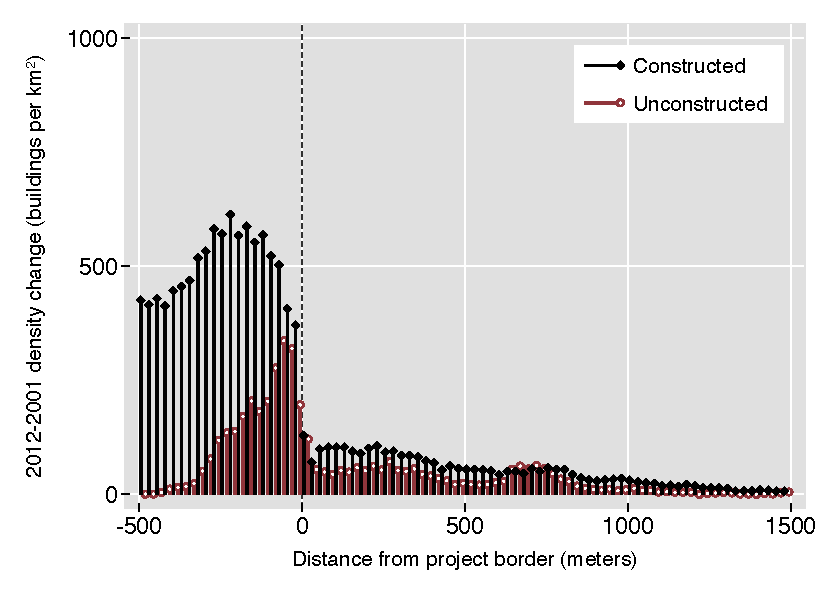
\includegraphics[width=\textwidth,trim={0.3cm .3cm 0.1cm 0cm}, clip=true]{figures/bblu_for_rawchanges_4_1_spk.pdf}

        \end{subfigure}
        \hfill
        \begin{subfigure}[b]{0.48\textwidth}  
                    \caption[]%
            {{\footnotesize \textbf{Greenfield} changes informal raw data }}     
            \label{fig:preinf}
            \centering 
            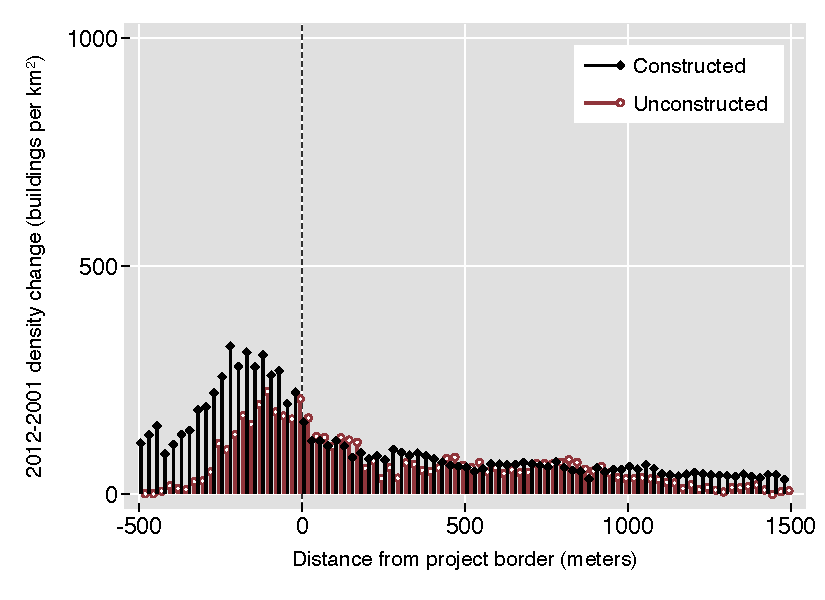
\includegraphics[width=\textwidth,trim={0.3cm .3cm 0.1cm 0cm}, clip=true]{figures/bblu_inf_rawchanges_4_1_spk.pdf}

        \end{subfigure}
        \begin{subfigure}[b]{0.48\textwidth}
                    \caption[Network2]%
            {{\footnotesize \textbf{In-Situ} changes formal raw data }}   
            \label{fig:prefor}
            \centering
            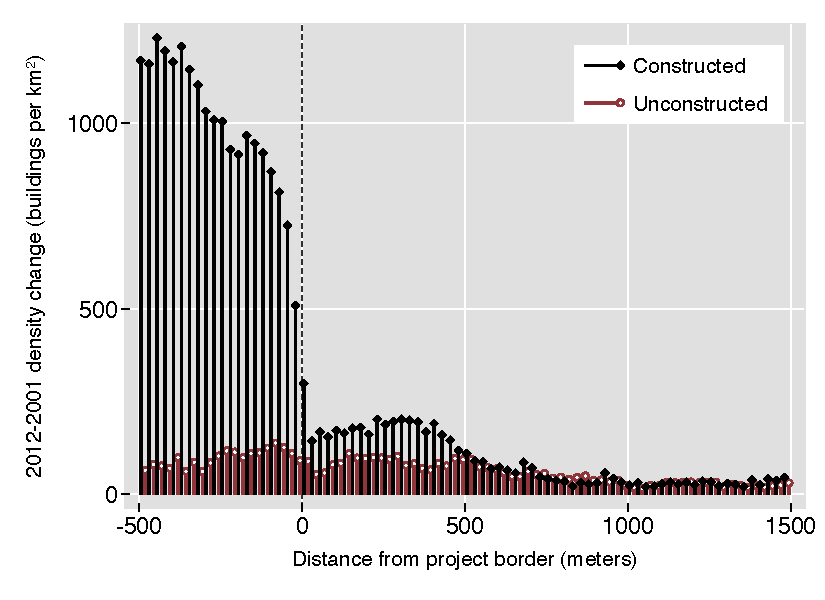
\includegraphics[width=\textwidth,trim={0.3cm .3cm 0.1cm 0cm}, clip=true]{figures/bblu_for_rawchanges_4_2_spk.pdf}

        \end{subfigure}
        \hfill
        \begin{subfigure}[b]{0.48\textwidth}  
                    \caption[]%
            {{\footnotesize \textbf{In-Situ} changes informal raw data }}     
            \label{fig:preinf}
            \centering 
            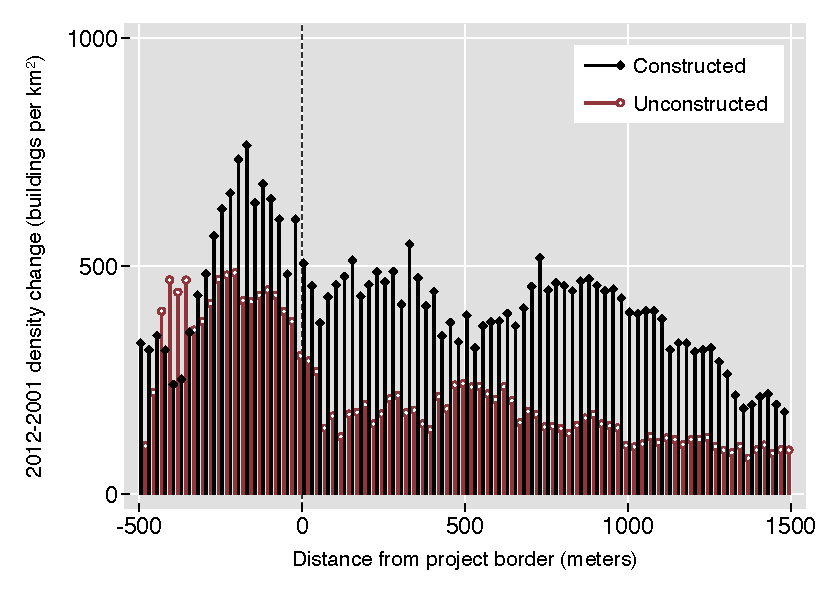
\includegraphics[width=\textwidth,trim={0.3cm .3cm 0.1cm 0cm}, clip=true]{figures/bblu_inf_rawchanges_4_2_spk.pdf}

        \end{subfigure}
        \begin{subfigure}[b]{0.48\textwidth}
                    \caption[Network2]%
            {{\footnotesize \textbf{Other} changes formal raw data}}   
            \label{fig:prefor}
            \centering
            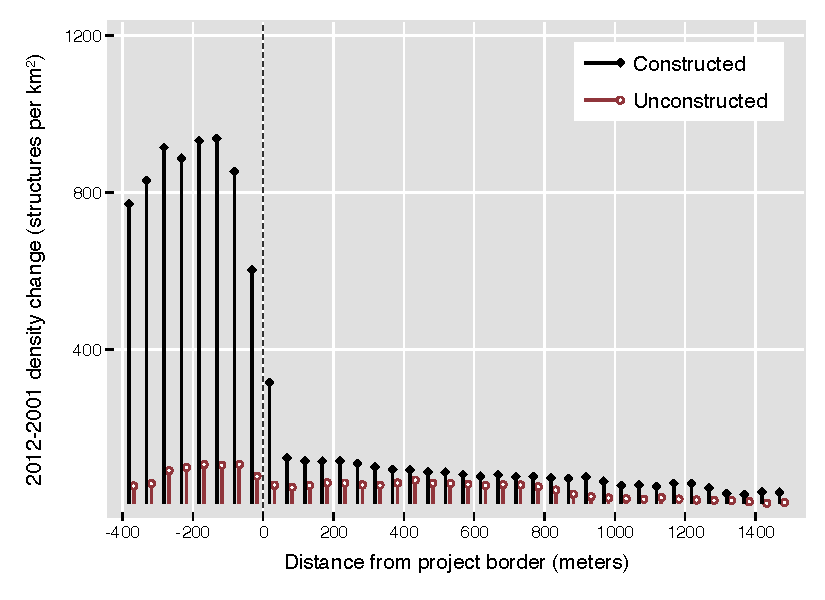
\includegraphics[width=\textwidth,trim={0.3cm .3cm 0.1cm 0cm}, clip=true]{figures/bblu_for_rawchanges_4_3_spk.pdf}

        \end{subfigure}
        \hfill
        \begin{subfigure}[b]{0.48\textwidth} 
                    \caption[]%
            {{\footnotesize \textbf{Other} changes informal  raw data}}      
            \label{fig:preinf} 
            \centering 
            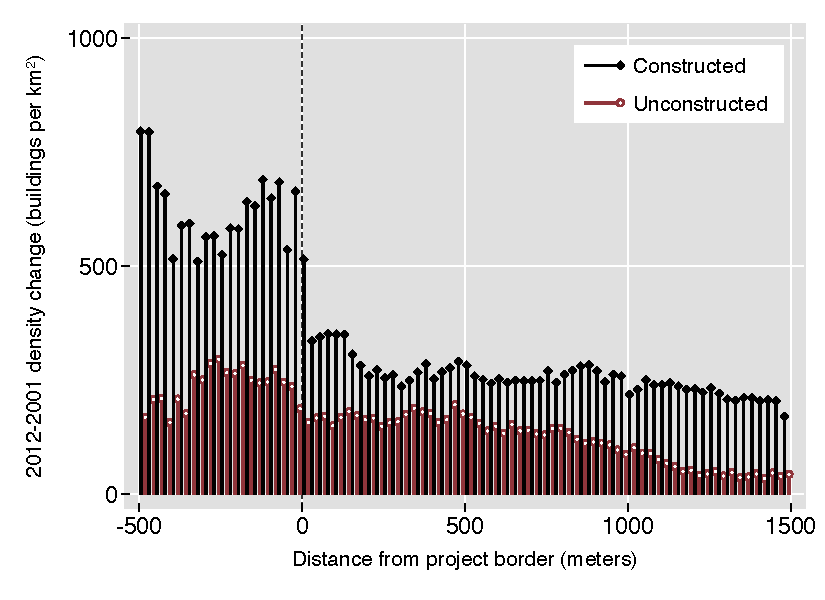
\includegraphics[width=\textwidth,trim={0.3cm .3cm 0.1cm 0cm}, clip=true]{figures/bblu_inf_rawchanges_4_3_spk.pdf}

        \end{subfigure}
\end{figure*}




\begin{figure*}
        \centering
   %     \caption[ Pre-Period Housing Densities in Constructed and Unconstructed Projects Areas ]
  %      {\small Pre-Period Densities} 
        %\vspace{2mm}
        \begin{subfigure}[b]{0.48\textwidth}
            \caption[Network2]%
            {{\footnotesize \textbf{All Projects} changes formal fe }}    
            \label{fig:prefor}
            \centering
            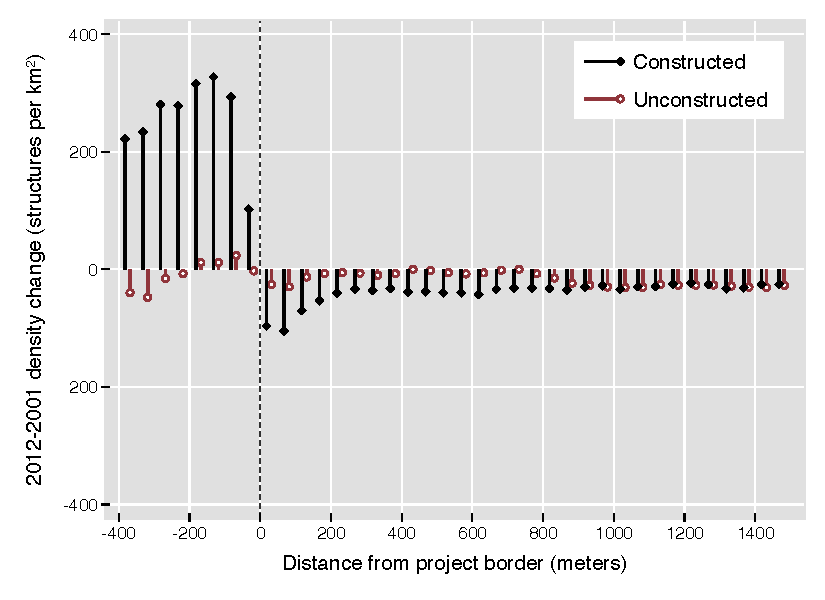
\includegraphics[width=\textwidth,trim={0.3cm .3cm 0.1cm 0cm}, clip=true]{figures/bblu_for_fe_rawchanges_4_sp_postk.pdf}

        \end{subfigure}
        \hfill
        \begin{subfigure}[b]{0.48\textwidth}  
                    \caption[]%
            {{\footnotesize \textbf{All Projects} changes informal  fe }}      
            \label{fig:preinf}
            \centering 
            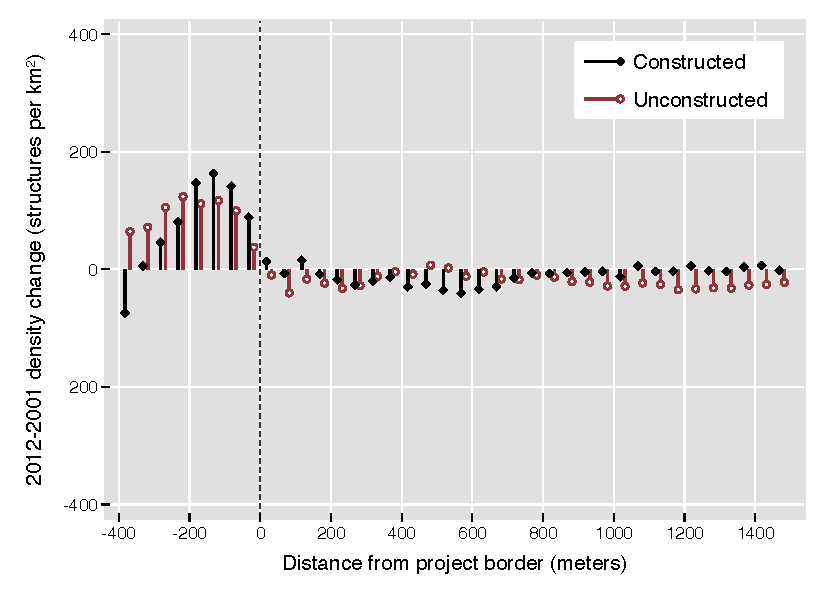
\includegraphics[width=\textwidth,trim={0.3cm .3cm 0.1cm 0cm}, clip=true]{figures/bblu_inf_fe_rawchanges_4_sp_postk.pdf}

        \end{subfigure}
        \begin{subfigure}[b]{0.48\textwidth}
                    \caption[Network2]%
            {{\footnotesize \textbf{Greenfield} changes formal  fe}}    
            \label{fig:prefor}
            \centering
            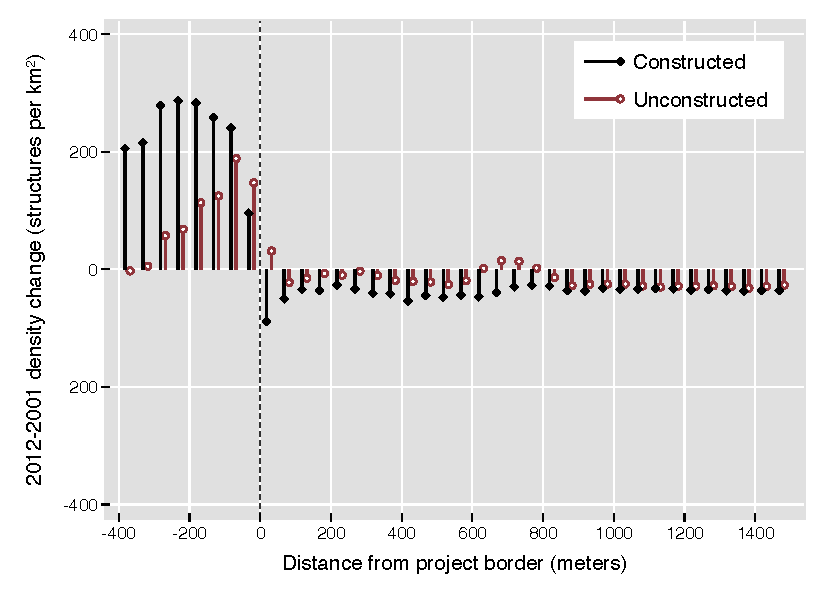
\includegraphics[width=\textwidth,trim={0.3cm .3cm 0.1cm 0cm}, clip=true]{figures/bblu_for_fe_rawchanges_4_1_sp_postk.pdf}

        \end{subfigure}
        \hfill
        \begin{subfigure}[b]{0.48\textwidth}  
                    \caption[]%
            {{\footnotesize \textbf{Greenfield} changes informal fe}}     
            \label{fig:preinf}
            \centering 
            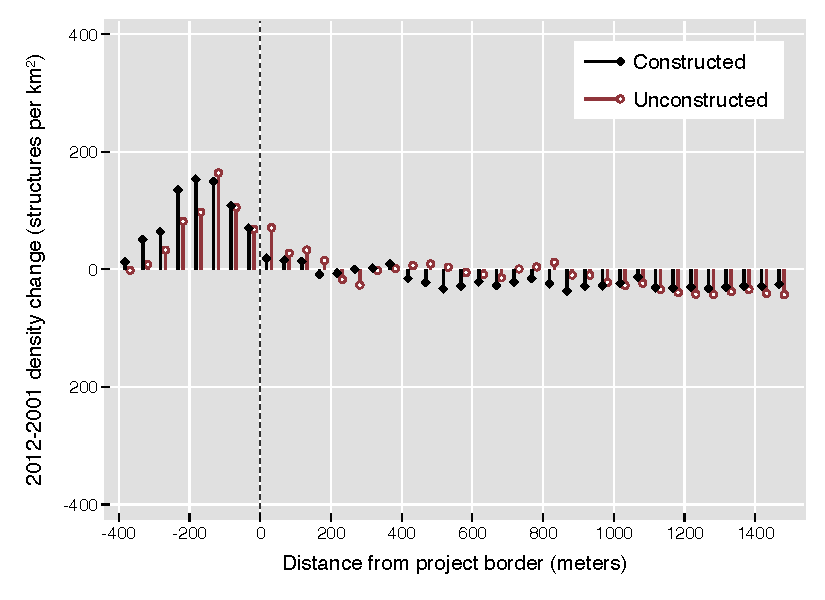
\includegraphics[width=\textwidth,trim={0.3cm .3cm 0.1cm 0cm}, clip=true]{figures/bblu_inf_fe_rawchanges_4_1_sp_postk.pdf}

        \end{subfigure}
        \begin{subfigure}[b]{0.48\textwidth}
                    \caption[Network2]%
            {{\footnotesize \textbf{In-Situ} changes formal fe}}   
            \label{fig:prefor}
            \centering
            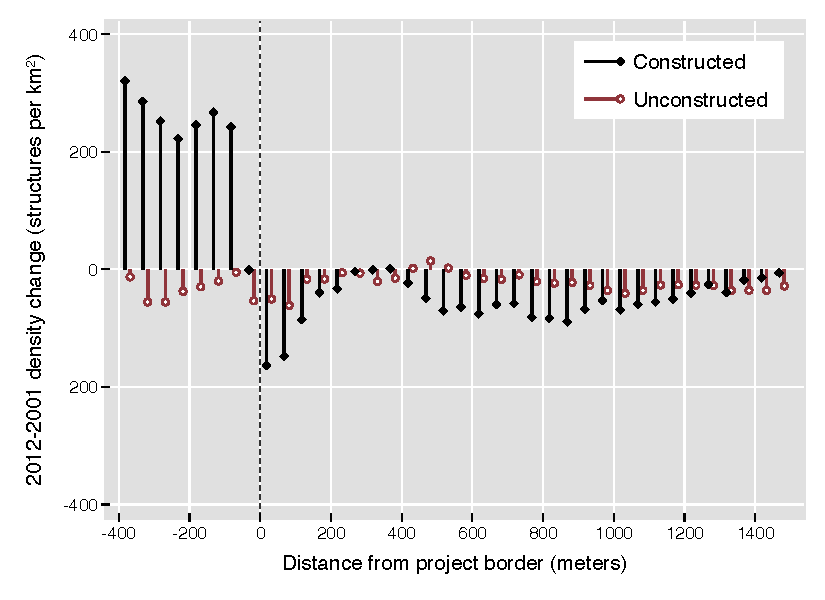
\includegraphics[width=\textwidth,trim={0.3cm .3cm 0.1cm 0cm}, clip=true]{figures/bblu_for_fe_rawchanges_4_2_sp_postk.pdf}

        \end{subfigure}
        \hfill
        \begin{subfigure}[b]{0.48\textwidth}  
                    \caption[]%
            {{\footnotesize \textbf{In-Situ} changes informal fe}}     
            \label{fig:preinf}
            \centering 
            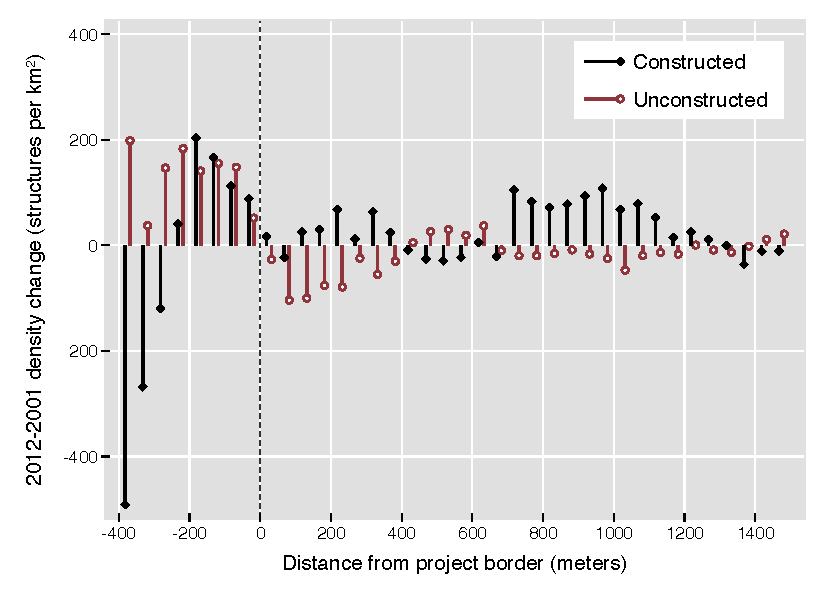
\includegraphics[width=\textwidth,trim={0.3cm .3cm 0.1cm 0cm}, clip=true]{figures/bblu_inf_fe_rawchanges_4_2_sp_postk.pdf}

        \end{subfigure}
        \begin{subfigure}[b]{0.48\textwidth}
                    \caption[Network2]%
            {{\footnotesize \textbf{Other} changes formal fe}}   
            \label{fig:prefor}
            \centering
            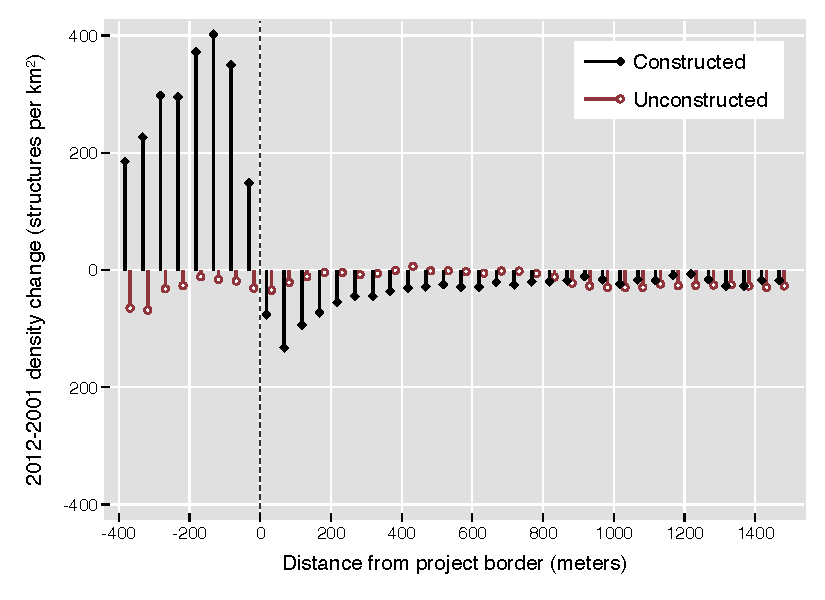
\includegraphics[width=\textwidth,trim={0.3cm .3cm 0.1cm 0cm}, clip=true]{figures/bblu_for_fe_rawchanges_4_3_sp_postk.pdf}

        \end{subfigure}
        \hfill
        \begin{subfigure}[b]{0.48\textwidth} 
                    \caption[]%
            {{\footnotesize \textbf{Other} changes informal  fe}}      
            \label{fig:preinf} 
            \centering 
            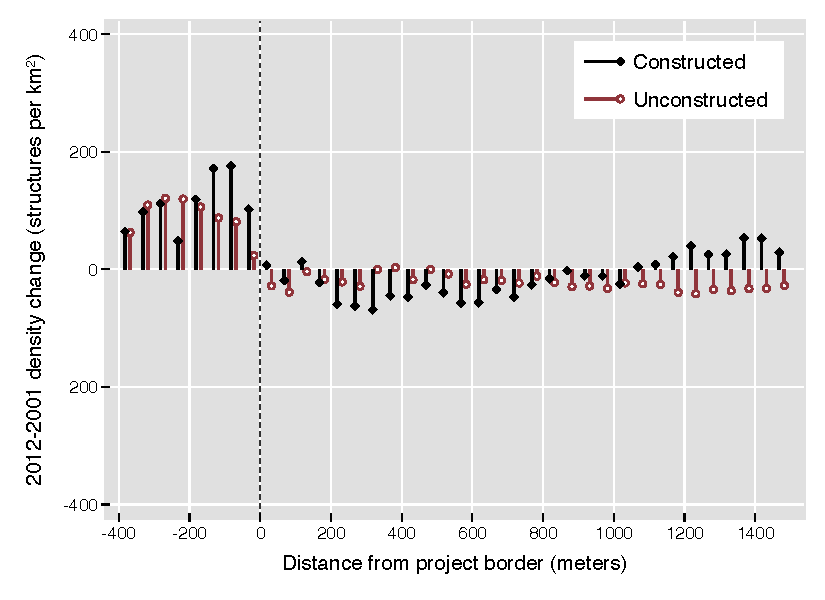
\includegraphics[width=\textwidth,trim={0.3cm .3cm 0.1cm 0cm}, clip=true]{figures/bblu_inf_fe_rawchanges_4_3_sp_postk.pdf}

        \end{subfigure}
\end{figure*}







\begin{table}
\caption{Building Density}
\begin{tabular}{lDDDDD}
\toprule
 & \small (1) & \small (2)  & \small (3) & \small (4) & \small (5) \\
 & Total & Formal  & Informal & Informal Bkyd. & Informal Non-Bkyd. \\ \midrule
\textbf{All Projects} \\inside project      &     442.949\textsuperscript{a}&     434.839\textsuperscript{a}&       8.110                   &     243.009\textsuperscript{a}&    -234.899\textsuperscript{a}\\
                    &   (141.525)                   &    (70.736)                   &   (102.611)                   &    (89.724)                   &    (71.576)                   \\[0.5em]
0-300m outside project &       9.716                   &       2.212                   &       7.504                   &     -27.462                   &      34.965                   \\
                    &    (45.467)                   &    (20.679)                   &    (38.401)                   &    (33.321)                   &    (26.349)                   \\[0.5em]
300-600m outside project &     -52.476\textsuperscript{c}&     -11.230                   &     -41.245\textsuperscript{c}&     -44.057\textsuperscript{b}&       2.811                   \\
                    &    (29.539)                   &    (12.167)                   &    (24.946)                   &    (20.673)                   &    (14.427)                   \\[0.5em]
R$^2$               &       0.442                   &       0.409                   &       0.405                   &       0.387                   &       0.346                   \\

\midrule
\textbf{Greenfield} \\   inside project      &     291.222                   &     225.343\textsuperscript{b}&      65.879                   &      95.480                   &     -29.601                   \\
                    &   (177.019)                   &   (111.203)                   &    (83.794)                   &    (80.862)                   &    (39.483)                   \\[0.01em]
0-300m outside project &     -12.347                   &     -14.572                   &       2.225                   &     -36.632                   &      38.857                   \\
                    &    (44.657)                   &    (21.170)                   &    (32.630)                   &    (26.130)                   &    (30.174)                   \\[0.01em]
300-600m outside project&     -15.206                   &      -8.119                   &      -7.087                   &     -21.488\textsuperscript{b}&      14.401                   \\
                    &    (29.727)                   &    (12.349)                   &    (24.961)                   &     (9.409)                   &    (20.726)                   \\[0.8em] 
\textbf{In-Situ Upgrading} \\   inside project      &     246.775                   &     593.950\textsuperscript{a}&    -347.174                   &      42.051                   &    -389.226                   \\
                    &   (624.187)                   &   (166.271)                   &   (512.677)                   &   (435.097)                   &   (321.209)                   \\[0.01em]
0-300m outside project &      94.218                   &      76.972                   &      17.246                   &     -80.646                   &      97.893                   \\
                    &   (230.769)                   &    (91.483)                   &   (185.316)                   &   (177.894)                   &   (117.059)                   \\[0.01em]
300-600m outside project &     -15.604                   &      35.262                   &     -50.866                   &    -120.741                   &      69.875                   \\
                    &   (105.433)                   &    (35.607)                   &    (96.393)                   &    (78.764)                   &    (66.237)                   \\[0.8em]
\textbf{Other} \\   inside project      &     701.477\textsuperscript{a}&     600.844\textsuperscript{a}&     100.633                   &     458.686\textsuperscript{a}&    -358.053\textsuperscript{a}\\
                    &   (140.062)                   &    (71.782)                   &   (106.875)                   &   (105.595)                   &    (87.664)                   \\[0.01em]
0-300m outside project &      -9.981                   &      10.392                   &     -20.374                   &     -28.477                   &       8.103                   \\
                    &    (63.378)                   &    (25.863)                   &    (55.802)                   &    (44.641)                   &    (32.911)                   \\[0.01em]
300-600m outside project &     -90.158\textsuperscript{c}&     -15.579                   &     -74.579\textsuperscript{c}&     -44.304                   &     -30.275\textsuperscript{c}\\
                    &    (47.772)                   &    (17.964)                   &    (40.994)                   &    (37.199)                   &    (15.514)                   \\[0.8em]
Mean Outcome 2001   &      526.22                   &      261.56                   &      264.66                   &       96.43                   &      168.23                   \\
Mean Outcome 2011   &      838.62                   &      385.14                   &      453.48                   &      286.79                   &      166.69                   \\
R$^2$               &       0.443                   &       0.411                   &       0.406                   &       0.388                   &       0.347                   \\
N                   &   1,705,534                   &   1,705,534                   &   1,705,534                   &   1,705,534                   &   1,705,534                   \\

\bottomrule
\end{tabular}
\end{table}





\begin{table}[h!] 
\caption{Effect of Housing Projects on Socio-demographics}
\label{table:sorting}
\small
\centering
%\caption{Census Composition Estimates }
\vspace{-2mm}
\begin{tabular}{lDDDDD}
\toprule
& \small (1) & \small (2) & \small (3) & \small (4)& \small (5)\\
& \small Age & \small P.O.B. not Gauteng & \small Unemployed & \small Years of Education & \small Monthly Income \\ \midrule 
\textbf{All Projects} \\inside project      &      -0.034                   &      -0.001                   &      -0.045\textsuperscript{b}&       0.197                   &     790.546                   \\
                    &     (0.401)                   &     (0.024)                   &     (0.022)                   &     (0.170)                   &   (582.267)                   \\[0.5em]
0-300m outside project &       0.384                   &      -0.010                   &      -0.022                   &       0.167                   &     273.665                   \\
                    &     (0.318)                   &     (0.017)                   &     (0.018)                   &     (0.122)                   &   (398.350)                   \\[0.5em]
300-600m outside project &      -0.005                   &      -0.007                   &      -0.009                   &      -0.054                   &     -87.509                   \\
                    &     (0.281)                   &     (0.015)                   &     (0.017)                   &     (0.120)                   &   (447.740)                   \\[0.5em]
R$^2$               &       0.703                   &       0.771                   &       0.528                   &       0.692                   &       0.666                   \\

\midrule
\textbf{Greenfield} \\   inside project      &      -0.259                   &      -0.015                   &       0.024                   &       0.597\textsuperscript{c}&    1318.206                   \\
                    &     (0.695)                   &     (0.062)                   &     (0.045)                   &     (0.353)                   &  (1033.803)                   \\[0.01em]
0-300m outside project &       0.105                   &       0.035                   &       0.037                   &      -0.076                   &     532.266                   \\
                    &     (0.834)                   &     (0.031)                   &     (0.042)                   &     (0.268)                   &   (625.183)                   \\[0.01em]
300-600m outside project&      -0.594                   &      -0.002                   &       0.022                   &       0.420\textsuperscript{c}&     361.354                   \\
                    &     (0.594)                   &     (0.028)                   &     (0.036)                   &     (0.241)                   &   (581.140)                   \\[0.8em] 
\textbf{In-Situ Upgrading} \\   inside project      &       0.852                   &       0.061                   &      -0.070\textsuperscript{b}&      -0.054                   &    -207.569                   \\
                    &     (0.600)                   &     (0.039)                   &     (0.028)                   &     (0.349)                   &  (1015.954)                   \\[0.01em]
0-300m outside project &       0.383                   &      -0.018                   &      -0.045                   &       0.237                   &    -165.918                   \\
                    &     (0.334)                   &     (0.026)                   &     (0.031)                   &     (0.252)                   &   (860.771)                   \\[0.01em]
300-600m outside project &      -0.004                   &       0.005                   &      -0.021                   &      -0.385\textsuperscript{c}&   -1267.956                   \\
                    &     (0.317)                   &     (0.028)                   &     (0.029)                   &     (0.216)                   &  (1168.354)                   \\[0.8em]
\textbf{Other} \\   inside project      &      -0.096                   &      -0.026                   &      -0.053\textsuperscript{c}&       0.174                   &    1014.926                   \\
                    &     (0.505)                   &     (0.034)                   &     (0.030)                   &     (0.209)                   &   (805.919)                   \\[0.01em]
0-300m outside project &       0.650                   &      -0.015                   &      -0.033                   &       0.128                   &     221.838                   \\
                    &     (0.453)                   &     (0.025)                   &     (0.022)                   &     (0.150)                   &   (584.719)                   \\[0.01em]
300-600m outside project &       0.361                   &      -0.017                   &      -0.019                   &      -0.117                   &     243.475                   \\
                    &     (0.430)                   &     (0.022)                   &     (0.023)                   &     (0.156)                   &   (547.037)                   \\[0.8em]
Mean Outcome 2001   &       27.30                   &        0.37                   &        0.47                   &        8.27                   &    2,477.01                   \\
Mean Outcome 2011   &       28.30                   &        0.43                   &        0.33                   &        9.68                   &    4,486.48                   \\
R$^2$               &       0.706                   &       0.774                   &       0.530                   &       0.695                   &       0.669                   \\
N                   &      12,734                   &      12,727                   &      12,724                   &      12,728                   &      12,724                   \\

\bottomrule
\multicolumn{6}{l}{\footnotesize Standard errors clustered at the project level in parenthesis. \textsuperscript{c} p$<$0.10, \textsuperscript{b} p$<$0.05, \textsuperscript{a} p$<$0.01  }\\
\multicolumn{6}{l}{\footnotesize P.O.B. means ``place of birth.''  Monthly income is in Rands.}
\end{tabular}
\end{table}








\begin{landscape}
{\footnotesize

\begin{table}[]
\small
\centering
\caption{Census Household-level Estimates }\label{table:censusestimates}
\vspace{-2mm}
\resizebox{.9\linewidth}{!}{
\begin{tabular}{lDDDDDDDD}
\toprule
 & \small (1) & \small (2)  & \small (3) & \small (4) & \small (5)  & \small (6)  & \small (7) & (8)\\
 & \small Flush Toilet & \small Water Indoors  & \small Electricity Cooking & \small Electricity Heating & \small Electricity Lighting  & \small Number of Rooms  & \small Household Size & Population Density\\ \midrule 
\textbf{All Projects} \\inside project      &       0.072                   &       0.166\textsuperscript{a}&       0.122\textsuperscript{b}&       0.100                   &       0.075                   &       0.187                   &       0.057                   &   -1452.735                   \\
                    &     (0.055)                   &     (0.052)                   &     (0.062)                   &     (0.061)                   &     (0.067)                   &     (0.209)                   &     (0.088)                   &  (1064.158)                   \\[0.5em]
0-300m outside project &      -0.000                   &       0.064                   &      -0.005                   &      -0.011                   &      -0.014                   &       0.022                   &      -0.068                   &   -1370.411                   \\
                    &     (0.036)                   &     (0.041)                   &     (0.037)                   &     (0.038)                   &     (0.038)                   &     (0.143)                   &     (0.063)                   &   (994.261)                   \\[0.5em]
300-600m outside project &      -0.033                   &       0.043                   &      -0.011                   &       0.002                   &      -0.025                   &      -0.078                   &      -0.019                   &   -1852.021                   \\
                    &     (0.026)                   &     (0.034)                   &     (0.024)                   &     (0.027)                   &     (0.024)                   &     (0.116)                   &     (0.053)                   &  (1549.353)                   \\[0.5em]
R$^2$               &       0.616                   &       0.594                   &       0.669                   &       0.634                   &       0.639                   &       0.676                   &       0.691                   &       0.607                   \\

\midrule
\textbf{Greenfield} \\   inside project      &       0.144                   &       0.136                   &       0.201                   &       0.068                   &       0.170                   &       0.704\textsuperscript{c}&       0.051                   &     313.256                   \\
                    &     (0.147)                   &     (0.144)                   &     (0.134)                   &     (0.147)                   &     (0.135)                   &     (0.384)                   &     (0.212)                   &  (2130.232)                   \\[0.01em]
0-300m outside project &      -0.021                   &       0.018                   &      -0.023                   &      -0.051                   &      -0.046                   &       0.093                   &       0.137                   &    -498.619                   \\
                    &     (0.088)                   &     (0.093)                   &     (0.069)                   &     (0.071)                   &     (0.059)                   &     (0.353)                   &     (0.136)                   &  (1417.443)                   \\[0.01em]
300-600m outside project&       0.025                   &       0.061                   &       0.022                   &       0.025                   &       0.025                   &       0.217                   &       0.126                   &   -6386.086                   \\
                    &     (0.064)                   &     (0.071)                   &     (0.041)                   &     (0.054)                   &     (0.035)                   &     (0.224)                   &     (0.095)                   &  (5426.145)                   \\[0.8em] 
\textbf{In-Situ Upgrading} \\   inside project      &       0.030                   &       0.111                   &       0.016                   &       0.067                   &      -0.104                   &      -0.143                   &      -0.083                   &   -2533.630                   \\
                    &     (0.110)                   &     (0.085)                   &     (0.129)                   &     (0.110)                   &     (0.136)                   &     (0.346)                   &     (0.148)                   &  (1743.211)                   \\[0.01em]
0-300m outside project &       0.059                   &       0.061                   &      -0.000                   &      -0.018                   &      -0.027                   &      -0.220                   &      -0.090                   &   -1842.691                   \\
                    &     (0.076)                   &     (0.080)                   &     (0.076)                   &     (0.074)                   &     (0.078)                   &     (0.237)                   &     (0.111)                   &  (1759.855)                   \\[0.01em]
300-600m outside project &      -0.034                   &       0.067                   &      -0.003                   &       0.021                   &      -0.053                   &      -0.290                   &      -0.049                   &     287.178                   \\
                    &     (0.065)                   &     (0.072)                   &     (0.059)                   &     (0.063)                   &     (0.065)                   &     (0.241)                   &     (0.104)                   &  (1506.585)                   \\[0.8em]
\textbf{Other} \\   inside project      &       0.057                   &       0.191\textsuperscript{a}&       0.142\textsuperscript{c}&       0.110                   &       0.135                   &       0.169                   &       0.126                   &   -1029.927                   \\
                    &     (0.074)                   &     (0.065)                   &     (0.084)                   &     (0.087)                   &     (0.089)                   &     (0.295)                   &     (0.114)                   &  (1171.214)                   \\[0.01em]
0-300m outside project &      -0.049                   &       0.080                   &      -0.026                   &      -0.012                   &      -0.022                   &       0.062                   &      -0.143\textsuperscript{c}&   -1322.910                   \\
                    &     (0.043)                   &     (0.057)                   &     (0.049)                   &     (0.050)                   &     (0.051)                   &     (0.191)                   &     (0.081)                   &  (1093.635)                   \\[0.01em]
300-600m outside project &      -0.053\textsuperscript{c}&       0.040                   &      -0.011                   &       0.007                   &      -0.016                   &      -0.066                   &      -0.065                   &   -1600.918\textsuperscript{c}\\
                    &     (0.031)                   &     (0.046)                   &     (0.030)                   &     (0.033)                   &     (0.030)                   &     (0.155)                   &     (0.068)                   &   (959.961)                   \\[0.8em]
Mean Outcome 2001   &        0.79                   &        0.35                   &        0.66                   &        0.62                   &        0.77                   &        3.30                   &        3.51                   &    8,566.83                   \\
Mean Outcome 2011   &        0.83                   &        0.54                   &        0.81                   &        0.72                   &        0.82                   &        3.56                   &        3.18                   &    9,823.82                   \\
R$^2$               &       0.627                   &       0.603                   &       0.675                   &       0.640                   &       0.645                   &       0.680                   &       0.694                   &       0.610                   \\
N                   &      12,732                   &      12,732                   &      12,732                   &      12,732                   &      12,732                   &      12,709                   &      12,730                   &      12,734                   \\

\bottomrule
\multicolumn{9}{l}{\footnotesize All regressions include 3km grid Fixed-Effects. Standard errors clustered at the project level in parenthesis. \textsuperscript{c} p$<$0.10,\textsuperscript{b} p$<$0.05,\textsuperscript{a} p$<$0.01 }
\end{tabular}
}
\end{table}

}
\end{landscape}




\begin{table}
\small
\centering
\caption{Triple Difference Estimates on Log-Prices}\label{table:priceDDD_het}
\vspace{-2mm}
\begin{tabular}{lCC}
\toprule
 & \small (1) & \small (2)  \\ \midrule 
 \textbf{All Projects} \\
 inside project      &      -0.183                   &      -0.168                   \\
                    &     (0.270)                   &     (0.266)                   \\[0.55em]
0-300m outside project &      -0.057                   &      -0.048                   \\
                    &     (0.065)                   &     (0.064)                   \\[0.5em]
300-600m outside project &      -0.008                   &      -0.007                   \\
                    &     (0.057)                   &     (0.057)                   \\[0.5em]
Lot Size Controls   &                               &  \checkmark                   \\
r2                  &        0.52                   &        0.52                   \\
N                   &      67,751                   &      67,751                   \\

 \midrule
\textbf{Greenfield} \\   inside project      &       0.051                   &      -0.080                   \\
                    &     (0.233)                   &     (0.233)                   \\[0.01em]
0-300m outside project &      -0.008                   &       0.005                   \\
                    &     (0.182)                   &     (0.179)                   \\[0.01em]
300-600m outside project&      -0.118                   &      -0.118                   \\
                    &     (0.151)                   &     (0.151)                   \\[0.8em]
\textbf{In-Situ Upgrading} \\   inside project      &       0.029                   &       0.090                   \\
                    &     (0.332)                   &     (0.303)                   \\[0.01em]
0-300m outside project &      -0.233\textsuperscript{b}&      -0.229\textsuperscript{b}\\
                    &     (0.104)                   &     (0.102)                   \\[0.01em]
300-600m outside project &      -0.106                   &      -0.105                   \\
                    &     (0.102)                   &     (0.104)                   \\[0.8em]
\textbf{Other} \\   inside project      &      -0.355                   &      -0.314                   \\
                    &     (0.323)                   &     (0.316)                   \\[0.01em]
0-300m outside project &      -0.021                   &      -0.017                   \\
                    &     (0.094)                   &     (0.093)                   \\[0.01em]
300-600m outside project &       0.007                   &       0.004                   \\
                    &     (0.077)                   &     (0.077)                   \\[0.8em]
Lot Size Controls   &                               &  \checkmark                   \\
r2                  &        0.52                   &        0.52                   \\
N                   &      67,751                   &      67,751                   \\

\bottomrule
\multicolumn{3}{l}{\footnotesize Standard errors clustered at the project level in parenthesis.} \\
\multicolumn{3}{l}{ \textsuperscript{c} p$<$0.10,\textsuperscript{b} p$<$0.05,\textsuperscript{a} p$<$0.01 }
\end{tabular}
\end{table} 

% \begin{figure}
% 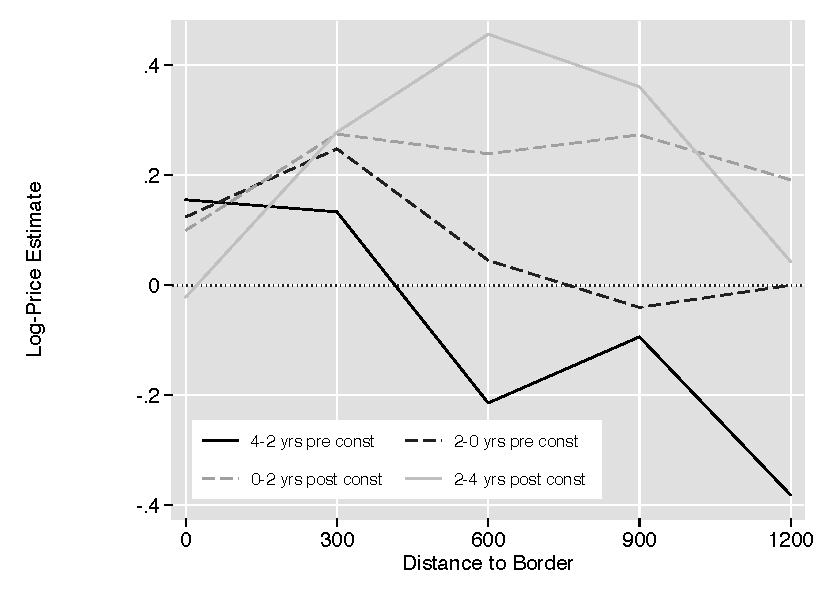
\includegraphics{figures/price_to_event_30.pdf}
% \end{figure}


\end{document}


